\documentclass[a4paper,10pt]{article}

%A Few Useful Packages
\usepackage{marvosym}
\usepackage{url,parskip}			%formatting
\usepackage[utf8]{inputenc} 
\usepackage{multirow}

%Graphics - Colors
\RequirePackage{color,graphicx}
\usepackage[usenames,dvipsnames]{xcolor}
% %better formatting of the A4 page
\usepackage[big]{layaureo}
%An alternative to Layaureo can be usepackage{fullpage}
 
\usepackage{supertabular} 		%for Grades
\usepackage{titlesec}			%custom section
 
%Setup hyperref package, and colours for links
\usepackage{hyperref}
\definecolor{linkcolour}{rgb}{0,0.2,0.6}
\hypersetup{colorlinks,breaklinks, urlcolor=linkcolour, linkcolor=linkcolour}

% \pagestyle{empty} % non-numbered pages
\usepackage[english]{babel}
\usepackage{slantsc}
\usepackage{array}
\usepackage{amsmath}

%FONTS
\usepackage[T1]{fontenc}
%\usepackage{arev}
%\newcommand{\fancyfont}{\fontfamily{avec}\selectfont}

%CV Sections inspired by:
%http://stefano.italians.nl/archives/26
\titleformat{\section}{\Large\scshape\raggedright}{}{0em}{}[\titlerule]
\titlespacing{\section}{0pt}{3pt}{3pt}

%XeTeX
%\usepackage{fontspec}			%load fonts
%\usepackage{xunicode,xltxtra} 	%other packages for XeTeX
%\defaultfontfeatures{Mapping=tex-text}
%\setmainfont[SmallCapsFont = Fontin SmallCaps]{Fontin}


%workEntry(end time, start time, job position, company, description)
\newcommand{\workEntry}[5]{
\begin{tabular}{p{1.7cm}|p{11cm}}
\raggedleft \textsc{#1} & #3 \\
\raggedleft \textsc{#2} & \emph{#4} \\
& \footnotesize{#5}\\
\multicolumn{2}{c}{}\ %this clears the space between two jobs
%some other job here
\end{tabular}
}

\newcommand{\dateEntry}[4]{
\begin{tabular}{p{1.7cm}|p{11cm}}
\raggedleft \textsc{#1} & #3 \\
\raggedleft \textsc{#2} & \footnotesize{#4}\\
\multicolumn{2}{c}{}\ %this clears the space between two jobs
%some other job here
\end{tabular}
}

\newcommand{\resEntry}[1]{
\begin{tabular}{p{1.7cm}|p{11cm}}
& #1 \\
\multicolumn{2}{c}{}\
\end{tabular}
}

\newcommand{\resEntryD}[2]{
\begin{tabular}{p{1.7cm}|p{11cm}}
& #1 \\
& \emph{#2} \\
\multicolumn{2}{c}{}\
\end{tabular}
}

\begin{document}

\par{\centering
{\huge{\textsc{Mart\'in A. Miguel}} }
\bigskip\par}

%Section: Personal Data
\section{Personal Data}
\begin{tabular}[c]{rp{7.5cm}r}
\textsc{Date of Birth:} & June $10^{th}$ 1990 & \multirow{4}{*}{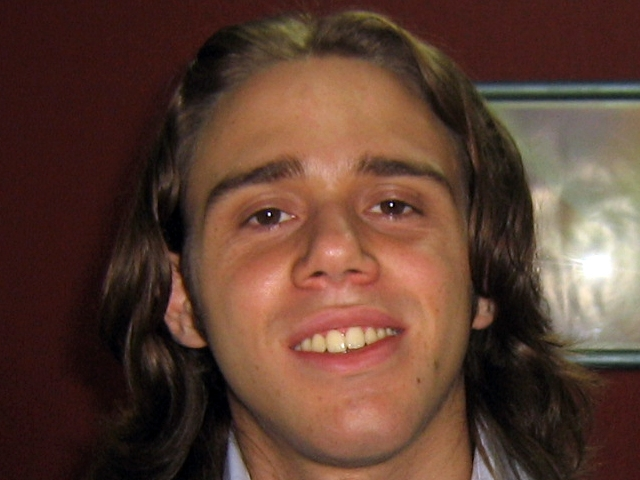
\includegraphics[scale=0.17]{../MMiguel-foto.jpeg}}\\
\textsc{Location:}	& Almagro, Capital Federal, \newline Buenos Aires, Argentina & \\
\textsc{Phone:}	& 4983-4768 15-3181-6018 & \\
\textsc{email:}	& \href{mailto:m2.march@gmail.com}{m2.march@gmail.com} & \\

\end{tabular}

%Section: Objective
\section{Objective}
My current professional objective focuses on the development of my personal skills. I am interested in testing my capability to face different kinds of situations, involving both technical and personal challenges. I look forward to contributing in projects, specially those where creativity is required, giving use to the knowledge and experience acquired throughout my studies and career.

%Section: Profile
\section{Professional/Personal Profile}
\begin{itemize}
 \item Analytical, efficiency-seeker
 \item Methodical, reliable 
 \item Curious, investigator, innovator
 \item Well-mannered, affable, thoughtful
\end{itemize}

%Section: Work Experience
\section{Work Experience}
\workEntry{Today}{August 2012}{Programador Java}{Despegar.com}{}

\workEntry{July 2012}{March 2011}{Assistant Teacher at UBA Computer Science course}{Universidad de Buenos Aires - FCEyN}{}

\workEntry{January 2010}{January 2009}{Jr. Java Programmer (J2ME / Blackberry)}{SenseByte}{}


%Section: Education
\section{Education}
\workEntry{2012}{2009}{Computer Science}{Universidad de Buenos Aires - FCEyN}%
{15 subjects completed}

\dateEntry{2008}{}{Compulsory Pre-University Course (CBC)}%
{Finished}

\workEntry{2007}{2003}{Comunication Oriented Bachelorship}{Instituto SUMMA}{}

\section{English Studies - Advanced Level}
\workEntry{2006}{}{FCE - First Certificate in English}{AACI}{Grade A\newline
\hspace*{0.15cm} \emph{University of Cambridge, ESOL Examinations}}

\workEntry{2004}{}{CILE 3 - English Certificate}{Facultad de Filosof\'ia y Letras, UBA}%
{Score: 80/100}

\section{Techology Knowledge}
\resEntry{Experienced in the following programming lenguages: C, C++, Java, Groovy, Python, Intel x86 Assembler, Haskell, ActionScript 2.0}{}

\resEntry{Knowledge on the following technologies: LaTeX, Octave}{}

\resEntry{Graphic and web design tools expertise: Adobe Photoshop, Adobe Flash}{}

\resEntry{Familiar with both Microsoft and Linux OS Technologies (Windows, Ubuntu)}{}

\section{IT Achievements}

\resEntry{Research work on algorithm optimisation using SIMD (Intel's SEE instruction set)}{}

\resEntry{Research work on heuristics methods to play a Zero-Sum board game}{}

\resEntry{Development of a basic monolithic kernel for x86 architecture based on UNIX ideas}{}

\resEntry{Experience on 3-stage software development starting on model specification in a theoretical level, %
moving to data structures definition in order to meet complexity restrictions, finishing in actual implementation %
of the defined code.}

%\section{Other Knowledge \& Studies}
%\workEntry{2008}{}{``Java Standard Programming, J2SE 5.0'' Course}{Educaci\'on IT Training Center}{Length: 40hs}
%
%\workEntry{2005}{}{``Action Script 2.0'' Course}{DaVinci Institute}{Length: 16hs}

% \resEntry{Software \& Hardware computer environment expertise}{}

%\section{Personal Achievements}
%\dateEntry{2007}{2006}{Year and a half working as speaker on a local radio}{}

%\dateEntry{2003}{}{First prize at school's literature competition}{}

\section{References}
\resEntryD{\textbf{Lic. Leandro Gleizer}}%
{Journalism, Radio and TV Teacher \newline
\href{mailto:leandrogleizer@hotmail.com}{leandrogleizer@hotmail.com}}\\

\resEntryD{\textbf{Gizzela Colona}}%
{AACI English Teacher \newline
\href{mailto:gizzella32@yahoo.co.uk}{gizzella32@yahoo.co.uk}}\\

\end{document}
